\documentclass[letterpaper,10pt]{article}
\usepackage[top=2cm, bottom=1.5cm, left=1cm, right=1cm]{geometry}
\usepackage{amsmath, amssymb, amsthm,graphicx}
\usepackage{fancyhdr}
\pagestyle{fancy}

\lhead{\today}
\chead{MV Stats Assignment 8}
\rhead{Justin Hood}

\newcommand{\Z}{\mathbb{Z}}
\newcommand{\Q}{\mathbb{Q}}
\newcommand{\R}{\mathbb{R}}
\newcommand{\C}{\mathbb{C}}
\newtheorem{lem}{Lemma}

\begin{document}
\begin{description}
\item[8.2] We consider the covariance matrix,
\[\Sigma= \begin{bmatrix}
5 & 2\\2 & 2
\end{bmatrix} \]
To start, we compute the correlation matrix $\rho$ as,
\[\rho=\begin{bmatrix}
1 & 2/\sqrt{10}\\2/\sqrt{10} & 1
\end{bmatrix} \]
We then compute the eigenvalues and eigenvectors of this matrix,
\begin{align*}
\lambda_1 &= \frac{2+\sqrt{1.6}}{2}\\
&\approx 1.63245\\
e_1 &= \begin{bmatrix}
\sqrt{2}/2\\\sqrt{2}/2
\end{bmatrix}\\
\lambda_2 &= \frac{2-\sqrt{1.6}}{2}\\
&\approx 0.367544\\
e_2 &= \begin{bmatrix}
\sqrt{2}/2\\-\sqrt{2}/2
\end{bmatrix}
\end{align*}
We then use this PCA analysis to write the principal components as,
\begin{align*}
Y_1 &= e_1'X\\
&=\frac{\sqrt{2}}{2}Z_1+\frac{\sqrt{2}}{2}Z_2\\
Y_2 &= e_2'X\\
&=\frac{\sqrt{2}}{2}Z_1-\frac{\sqrt{2}}{2}Z_2\\
\end{align*}
We then consider the proportion of the variance that is explained by $Y_1$ as,
\[\frac{\lambda_1}{\lambda_1+\lambda_2}=\frac{1.6325}{2}=0.8162278\]
We now consider the same PCA on $\Sigma$. Here, we find,
\begin{align*}
Y_1&=0.8944272X_1+0.4472136X_2\\
Y_2&=0.4472136X_1-0.8944272X_2
\end{align*}
and,
\[\frac{\lambda_1}{\lambda_1+\lambda_2}=\frac{6}{7}=0.8571429\]
We see here that the PC's computed between the two matrices are different. This is to be expected, as our matrices have much different variances.\\
Finally, we compute,
\begin{align*}
\rho_{Y_1,Z_1} &= e_{11}\sqrt{\lambda_1}\\
&=\frac{\sqrt{2}}{2}\sqrt{1.6325}\\
&=0.9034532\\
\rho_{Y_1,Z_2} &= e_{12}\sqrt{\lambda_1}\\
&=\frac{\sqrt{2}}{2}\sqrt{1.6325}\\
&=0.9034532\\
\rho_{Y_2,Z_1} &= e_{21}\sqrt{\lambda_2}\\
&=\frac{\sqrt{2}}{2}\sqrt{0.368}\\
&=0.4286866\\
\end{align*}
\item[8.6] We now consider the data from 4.12.
\[\bar{X}=\begin{bmatrix}
155.60\\14.70
\end{bmatrix},\ S=\begin{bmatrix}
7476.45 & 303.62\\303.62 & 26.19
\end{bmatrix} \]
We compute,
\begin{align*}
\lambda_1 &= 7488.80293\\
e_1 &= \begin{bmatrix}
0.99917337\\0.04065185
\end{bmatrix}\\
\lambda_2 &= 13.83707\\
e_2 &= \begin{bmatrix}
0.04065185\\ -0.99917337
\end{bmatrix}
\end{align*}
Our principle components are then,
\begin{align*}
y_1 &= 0.99917337x_1+0.04065185x_2\\
y_2 &= 0.04065185x_1+0.99917337x_2
\end{align*}
To find the proportion of the variance explained by $y_1$ we compute,
\[\frac{\lambda_1}{\lambda_1+\lambda_2}=\frac{7488.80293}{7488.80293+13.83707}=0.998155706\]
Next, we sketch the constant density ellipse,
\[(x-\bar{x})'S^{-1}(x-\bar{x})=1.4\]
\begin{center}
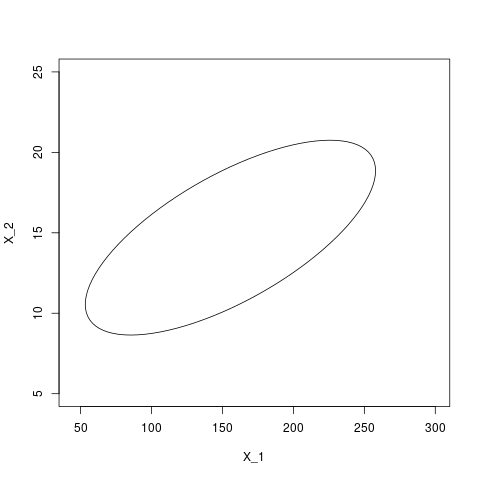
\includegraphics[scale=.75]{ellip.png}
\end{center}
Here, the principle components are the major and minor axes of the ellipse respectively.(I could not get the plot to cooperate).\\
Then, we compute the corrleation matrix,
\[R=\begin{bmatrix}
1 & 0.6861434\\ 0.6861434 & 1
\end{bmatrix} \]
As such, we see that,
\begin{align*}
r_{y_1,x_1} &= 1\\
r_{y_1,x_2} &= 0.6861434
\end{align*}
These values imply that the first component is almost entirely comprised of the sales data. Its variance is much greater than the profit variable.
\item[8.7] Using $R$, we compute the component analysis on the R matrix from before,
\begin{align*}
\lambda_1 &= 1.6861434\\
e_1 &= \begin{bmatrix}
\sqrt{2}/2\\\sqrt{2}/2
\end{bmatrix}\\
\lambda_2 &= 0.3138566\\
e_2 &= \begin{bmatrix}
\sqrt{2}/2\\ -\sqrt{2}/2
\end{bmatrix}
\end{align*}
Thus,
\begin{align*}
y_1 &= \frac{\sqrt{2}}{2}x_1+\frac{\sqrt{2}}{2}x_2\\
y_2 &= \frac{\sqrt{2}}{2}x_1-\frac{\sqrt{2}}{2}x_2
\end{align*}
The variances for each of these components are $\lambda_1$ and $\lambda_2$ respectively. As such, we can compute the proportion of variance explained by $y_1$ as,
\[\frac{1.6861434}{2}=0.8430717\]
Our sample correlation coefficients are then,
\begin{align*}
r_{y_1z_1} &= e_{11}\sqrt{\lambda_1}\\
&=0.9181894\\
r_{y_1z_2} &= e_{12}\sqrt{\lambda_1}\\
&=0.9181894\\
\end{align*}
So, we see that the standardized sales and profits are equal contributors in the first component. From 8.6, we saw that the sales variable were both larger values, and had a higher variance than the profit variable. As such we saw the $x_1$ variable dominated the PCA from the covariance matrix. After normalizing the data with the correlation matrix, we saw that the two components were roughly equal. This method is more likely the better of the two, as it does not allow for the artificially high variance in one of the variables to dominate the analysis.
\item[8.11] We consider the Census-tract data. First, we compute the covariance matrix for the data, after scaling the last column by a factor of 10. The result is,
\[S=\begin{bmatrix}
3.3968990 &  -1.102139  &   4.3055548  &  -2.078285  &  0.2720391\\
-1.1021394  &  9.672775  &  -1.5132363  &  10.953232 &  12.0306366\\
4.3055548 &  -1.513236  &  55.6259116 &  -28.937464 &  -0.4355907\\
-2.0782852 &  10.953232  & -28.9374642   & 89.066612  &  9.5729973\\
0.2720391 &  12.030637  &  -0.4355907  &   9.572997 &  31.8625082
\end{bmatrix} \]
We see that this is the same as the matrix from example 8.3, with column and row 5 scaled by 10, and the fifth diagonal scaled by 100. The scaling of 10 in the rows and columns is simply a side effect of the linear scaling of the variable. The factor of 100 becomes apparent from the equation,
\[\frac{1}{n}\sum(x_{ji}-\bar{x}_i)(x_{jk}-\bar{x}_j)\]
For the scaled variable, we have the form,
\[\frac{1}{n}\sum(10x_{55}-10\bar{x}_5)(10x_{55}-10\bar{x}_5)=\frac{100}{n}\sum(10x_{55}-10\bar{x}_5)(10x_{55}-10\bar{x}_5)\]
Hence the 100 factor.\\
Using $R$, we compute the first two principle components to be,
\begin{align*}
y_1 &= 0.03762881x_1-0.1189296x_2+0.4796729x_3-0.8589118x_4-0.1289352x_5\\
y_2 &= 0.06230915x_1 +0.249301x_2 +0.7596765x_3 +0.3163999x_4 +0.5067043x_5
\end{align*}
We then compute the cumulative proportion of variance explained by these components as,
\[\frac{\lambda_1+\lambda_2}{\sum \lambda_i}=0.7984804\]
Next, we compute the following,
\begin{align*}
r_{y_1x_1} &= 0.2124404\\
r_{y_1x_2} &= -0.3978987\\
r_{y_1x_3} &= 0.6692133\\
r_{y_1x_4} &= -0.946998\\
r_{y_1x_5} &= -0.2376782\\
r_{y_2x_1} &= -0.2220491\\
r_{y_2x_2} &= -0.5264862\\
r_{y_2x_3} &= -0.6690038\\
r_{y_2x_4} &= -0.2202\\
r_{y_2x_5} &= -0.5895939
\end{align*}
Comparing this to example 8.3, we see that the first components values are not too far off, differences of less than one tenth. However, for the second component, the values are significantly different, especially $r_{22}$.
\item[8.14] To begin, we conider the covariance matrix,
\[S=\begin{bmatrix}
2.879 & 10.010 & -1.810\\
10.010 & 199.788 & -5.640\\
-1.810 & -5.640 & 3.628
\end{bmatrix} \]
From this covariance matrix, we also compute the eigenvalues/eigenvectors for our PCA. Before we consider the QQ plots, we look at a plot of the ratio of explained variance,
\begin{center}
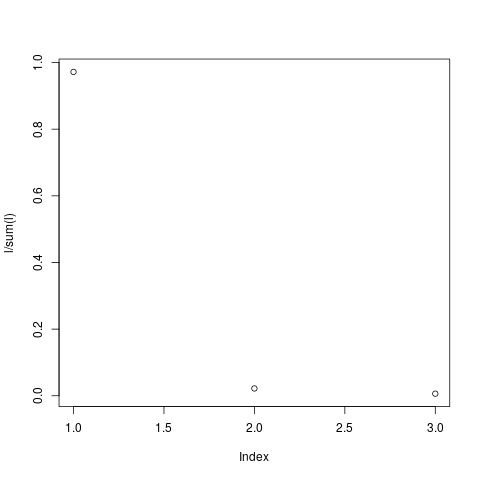
\includegraphics[scale=.75]{eigprop.png}
\end{center}
We see here that the first of the components is far more influential than the others. So, we consider its $QQ$ plot,
\begin{center}
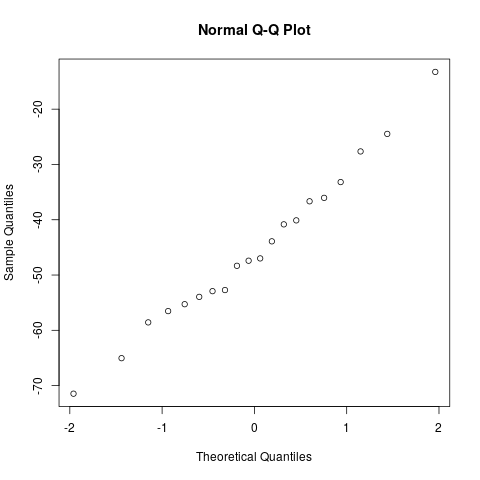
\includegraphics[scale=.75]{1qq.png}
\end{center}
We see that this plot is quite linear, and does not appear to have any extreme points or outliers.
\item[8.20] We consider the track record data. First, we import and construct the $S$ matrix. We also compute $\bar{X}$ as,
\[\bar{X}=[10.21685,\ 20.54148,\ 45.82907,\ 1.768148,\ 3.653333,\ 13.61759,\ 28.53519,\ 133.4785]\]
Computing the eigenvalues and vectors, we find the following regarding the cumulative proportions,
\begin{center}
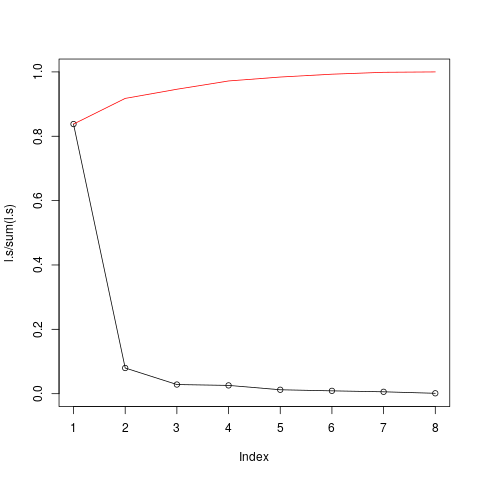
\includegraphics[scale=.75]{cumvval.png}
\end{center}
We see that the first PC accounts for roughly 84\% of the variance. Combining the first two components, we account for about 92\%. These components are,
\begin{align*}
y_1 &=0.33238773x_1+0.346051060x_2 +0.339124019x_3+ 0.35301338x_4+ \\
& 0.36598491x_5+ 0.36982036x_6+ 0.36594893x_7+ 0.35427792x_8\\
y_2 &= -0.52939911x_1 -0.470390497x_2 -0.345329287x_3 + 0.08945523x_4+ \\
& 0.15365241x_5+  0.29475985x_6+  0.33360619x_7+  0.38656085x_8
\end{align*}
Looking at these two components, we see that all of the signs are the same for the first component. In this way, a nations records in a given event are cumulatively scaled and summed to provide a sort of metric for comparison. In this way, we could call this component the measurement of skill or altheticism. Looking at the second vector, we see that some of the components are negative, and the others are positive. Because the variables are ordered from shortest distance to longest, we see that this scaling helps to reduce false values from lack of scaling of the distances.\\
Finally, we consider comparing the nations based on the first component now. We compute $X\cdot e_1$, and then sort the countries based on their scores.
\[\begin{bmatrix}
U.S.A. & 85.63052\\
Kenya   & 85.81863\\
France   & 86.91273\\
GreatBritain  &  86.94300\\
Japan  &  87.06855\\
Brazil  &  87.06938\\
Belgium  &  87.18382\\
Australia  &  87.22922\\
Mexico  &  87.28480\\
Portugal  &  87.32580\\
Italy  &  87.33011\\
Spain  &  87.50262\\
Germany  &  87.58127\\
Netherlands  &  88.16301\\
Poland  &  88.19532\\
Russia   & 88.23536\\
Canada   & 88.40680\\
Korea,South  &  88.44795\\
NewZealand  &  88.54557\\
Switzerland  &  88.55869\\
Ireland  &  88.68066\\
China  &  88.77554\\
Norway  &  88.93878\\
Denmark  &  88.99931\\
Argentina  &  89.03377\\
Sweden  &  89.16637\\
Finland  &  89.28152\\
Greece  &  89.67693\\
Hungary  &  89.68289\\
CzechRepublic  &  89.73418\\
Austria  &  89.80797\\
Columbia  &  89.83993\\
Romania   & 89.92071\\
Chile  &  89.92317\\
Turkey  &  89.97282\\
Korea,North  &  90.15981\\
India  &  90.28064\\
CostaRica  &  91.31959\\
Israel  &  91.51816\\
Luxembourg  &  91.91272\\
Taiwan  &  91.92754\\
Guatemala  &  92.02638\\
Philippines  &  93.25636\\
Thailand  &  93.68469\\
Indonesia  &  93.79810\\
Mauritius  &  94.34089\\
Myanmar(Burma)  &  95.03512\\
DominicanRepub  &  95.90629\\
Bermuda  &  96.20086\\
Singapore  &  97.05492\\
Malaysia  &  97.30645\\
PapuaNewGuinea  &  98.14549\\
Samoa &  106.18833\\
CookIslands  & 110.88311
\end{bmatrix}\]
We see that this ranking matches conventional wisdom. This also matches the same analysis for the womens data as well.
\item[8.21] Again, we consider the track record data. We perform the same analysis as before, but after converting to speed, as opposed to time. The first two components are then,
\begin{align*}
y_{1} &= 0.2439701x_1 +0.3113827x_2 +0.316815066x_3 +0.27750476x_4\\ 
&+0.36426209x_5+0.42768607x_6+0.42091797x_7 +0.41637063x_8\\
y_{2} &= -0.4323711x_1 -0.5234562x_2 -0.469058273x_3 -0.03280175x_4 \\
& +0.06284374x_5+0.26134677x_6 + 0.30988613x_7+  0.38688033x_8
\end{align*}
Again, we see the same matching sign in the first component, and differing signs based on the distance in the second. Ranking the countries again based on the first component, we find similar results to the first, matching conventional wisdom,
\[\begin{bmatrix}
CookIslands & 17.34402\\
Samoa & 17.84922\\
PapuaNewGuinea & 18.96298\\
\vdots & \vdots\\
GreatBritain & 20.85006\\
Kenya & 20.93116\\
U.S.A. & 21.10820
\end{bmatrix}\]
Looking to choose the better of the two methods, we see that the two component analysis in 8.20 has a \% variance of $.9177$, whereas the speed analysis has $.92335$. Thus, we see that the speed data is slightly better. If we think about the meanings of the data that we are breaking into components, we note that ranking based on speed makes more sense for meaning in human terms, as a faster running country means more than a country with low times. 
\end{description}
\end{document}
